\documentclass[12pt]{article}

\usepackage[margin=1in]{geometry}
\usepackage{amsmath,amsthm,amssymb}

\newcommand{\N}{\mathbb{N}}
\newcommand{\Z}{\mathbb{Z}}
\newcommand{\homeworkheader}[2]{
  \title{Homework #1}
  \author{Erich Menge (X.500: menge053, Student ID: 4624713) \\
  #2}
  \maketitle
}

\newenvironment{problem}[1]{
  \ignorespaces
  \section*{Problem #1}
}{
  \ignorespacesafterend
}

\newcommand{\classnameandsection}{CSCI 4707 Practice of Database Systems}


\sethomeworknumber{5}

\begin{document}
\homeworkheader{\classnameandsection}

\begin{problem}{1}
  Let $T = \{(i,j,k) | i,j,k \text{ are natural numbers}\}$. Show that T is countable.
  \begin{solution}
    For each pair $(i,j) \in \mathbb{N}$ we can show a correspondence between $(i,j)$ as $f: \mathbb{N} \rightarrow
    \mathbb{N}$ \\
    See figure ~\ref{fig:problem_1_a}.
    \begin{figure}[H]
      \centering
      \caption{$f: \mathbb{N} \rightarrow \mathbb{N}$}
      \includegraphics[scale=.5]{problem_1_a.eps}
      \label{fig:problem_1_a}
    \end{figure}
    \noindent Then, if we let each unique pair $(i,j) = a, b, c, \ldots$ we can show a correspondence between those pairs and $k$.\\
    See figure ~\ref{fig:problem_1_b}.
    \begin{figure}[H]
      \centering
      \caption{$f: \mathbb{N} \times \mathbb{N} \rightarrow \mathbb{N}$}
      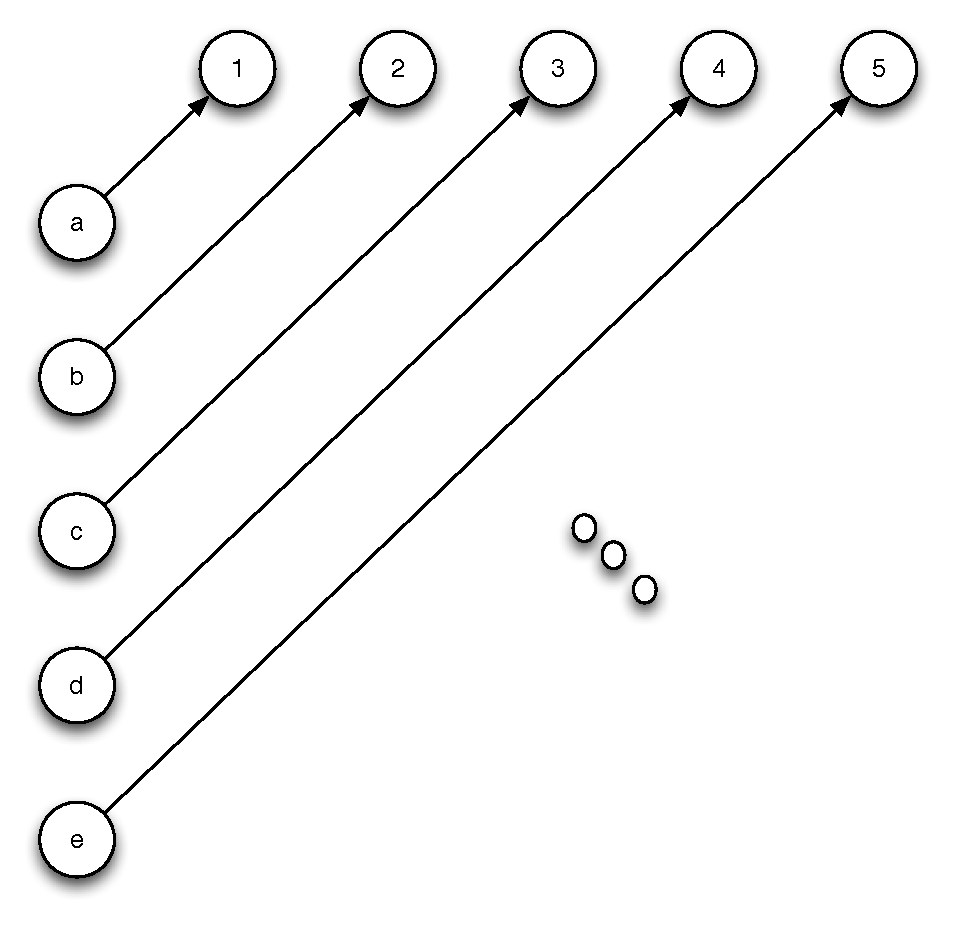
\includegraphics[scale=.5]{problem_1_b.eps}
      \label{fig:problem_1_b}
    \end{figure}
    Because $T$ is onto and one-to-one with $\mathbb{N}$ we can show that these sets are the same size and thus are
    countable.
  \end{solution}
\end{problem}

\begin{problem}{2}
\end{problem}

\begin{problem}{3}
\end{problem}

\begin{problem}{4}
\end{problem}

\begin{problem}{5}
\end{problem}

\begin{problem}{6}
\end{problem}

\begin{problem}{7}
\end{problem}


\end{document}
